\begin{filecontents}{preliminary.sty}
\ProvidesPackage{preliminary}
%\DeclareOption{draft}{%
  \AtBeginDocument{%
    \renewcommand\maketitlehookc
\ProcessOptions
\RequirePackage{titling}
\endinput
\end{filecontents}

\documentclass[pdftex,12pt, a4paper]{article}
\usepackage{setspace}
\usepackage{ragged2e}
\usepackage[centertags,reqno]{amsmath}
\usepackage{amssymb}
\usepackage{graphics,subfigure}
\usepackage[dvips]{graphicx}
\usepackage[dvipsnames]{xcolor}
\usepackage[hidelinks]{hyperref}
\usepackage{appendix}
\usepackage{natbib}
\usepackage{verbatim,color}
\usepackage{pdflscape}
\usepackage[showframe=false]{geometry}
\usepackage{changepage}
\usepackage{xcolor}
\definecolor{LightBlue}{rgb}{0.902, 0.945, 1}
\usepackage{mdframed}
\usepackage{eurosym}
\usepackage{textcomp}
\usepackage[open,openlevel=1]{bookmark}
\usepackage{multirow}
\usepackage{caption}
\usepackage{hyphenat}
\usepackage{listings} % To include a Stata .do file
\usepackage{pdfpages} % To include the instructions from a pdf file
\usepackage{tikz}
\newcommand{\mybox}[2]{{\color{#1}\fbox{\normalcolor#2}}}
\doublespacing

\usepackage{wasysym} % For radio buttons
\usepackage{tasks} % For items side by side, aligned in pairs
\usepackage{makecell} % Splits long text in table cell



% Exception to hyphenation
\hyphenation{par-ti-ci-pants}
\hyphenation{par-ti-ci-pant}
\hyphenation{Hy-po-the-sis}
\hyphenation{ex-pe-ri-ment}
\hyphenation{ex-pe-ri-ments}

% Allows bigger tables to be scaled down
\usepackage{adjustbox}

%From my paper with Raymond
\usepackage{tabularx,calc}
\usepackage{dcolumn}                    % Aligns tables on the decimal point
\newcolumntype{d}[1]{D{.}{.}{#1}}       %       Aligns on dot
\newcolumntype{.}{D{.}{.}{3.5}}         %       Somehow it works better
\newcolumntype{C}{@{\extracolsep{.6cm}}c@{\extracolsep{0pt}}}
\usepackage{threeparttable}
\usepackage{siunitx,booktabs}
\sisetup{
    detect-all,
    round-integer-to-decimal = true,
    group-digits             = true,
    group-minimum-digits     = 4,
    group-separator          = {\,},
    table-align-text-pre     = false,
    table-align-text-post    = false,
    input-signs              = + -,
    input-symbols            = {*},
    input-open-uncertainty   = ,
    input-close-uncertainty  = ,
    retain-explicit-plus
}

% Commands to name appendices Appendix A, Appendix B, etc.
\makeatletter
%% The "\@seccntformat" command is an auxiliary command
%% (see pp. 26f. of 'The LaTeX Companion,' 2nd. ed.)
\def\@seccntformat#1{\@ifundefined{#1@cntformat}%
   {\csname the#1\endcsname\quad}  % default
   {\csname #1@cntformat\endcsname}% enable individual control
}
\let\oldappendix\appendix %% save current definition of \appendix
\renewcommand\appendix{%
    \oldappendix
    \newcommand{\section@cntformat}{\appendixname~\thesection\quad}
}

%Adds text specifying it is a preliminary version
%\usepackage{preliminary}

\title{Testing the elicitation procedure \\ of the Minimum Acceptable Probability}
\author{Maria Polipciuc\thanks{WU Vienna University of Economics and Business and Maastricht University. Email: \url{maria.polipciuc@wu.ac.at}.} \and Martin Strobel\thanks{Maastricht University. We thank Elias Tsakas, Mats K\"{o}ster, Andrea Isoni and participants at the BEELab proposal meeting and the interdisciplinary brownbag seminar of behavioral sciences at Maastricht University, the 2022 M-BEES and the 2022 European ESA conferences, and the fall 2022 Berlin Behavioral Economics Workshop for valuable comments.}}
\date{\today	\vspace{1cm}}
\titlepage


\begin{document}
\begin{titlepage}
\clearpage
\maketitle
\thispagestyle{empty}


\begin{abstract}
%Betrayal aversion has been shown to be an important determinant of trust \citep{Bohnet2004}.
%Its original identification via Minimum Acceptable Probabilities (MAPs) allows for confounding factors to be mistaken for betrayal aversion \citep{Li2020a}.
%
%%We run an online experiment to estimate the impact of one potential confound: more pessimistic beliefs in the binary trust game compared to the control game.
%%\textcolor{red}{Participants have to state MAPs for preferring the outcome of a lottery (which will be selected at random from a set of lotteries) to a certain amount.
%%Across three treatments, the support for the lotteries is the same, but we vary the probability of each lottery to be selected.
%%--> I am thinking the text in red could be removed.}
%
%%We find that MAPs are lowest in the treatment with high mass on ``bad'' lotteries, followed by MAPs in an in-between (uniform) treatment, followed by MAPs in the treatment with high mass on ``good'' lotteries.
%In an experiment, we find that MAPs are lower the worse the prospects one faces.
%%The differences run opposite to what we expected: a lower MAP in the uniform as compared to the ``bad'' treatment.
%Underlying distributions (beliefs about them) influence valuation elicited through MAP, but in the opposite direction to the one we expected.
%This is similar to the distributional dependence of valuations elicited using the Becker--DeGroot--Marschak mechanism, which closely resembles how MAPs are elicited.

Betrayal aversion has been shown to be an important determinant of trust \citep{Bohnet2004}.
We study whether the way betrayal aversion is identified (as a difference in Minimum Acceptable Probabilities, MAPs) is affected by beliefs about one’s prospects.

In a within-subject design, we find that MAPs are lower the worse the prospects one faces.
This is similar to the distributional dependence of valuations elicited using the Becker–DeGroot–Marschak mechanism.
Our results suggest that distributional dependence should be accounted for when eliciting MAPs to isolate betrayal aversion.

\noindent \textit{JEL: C72, C81, C91}

\noindent  \textit{Keywords: Betrayal aversion, beliefs, reference, valuation}

\end{abstract}
\end{titlepage}


\section{Introduction}\label{sec:intro}
Individuals have often been found to prefer exposure to a randomly generated risk over exposure to an equiprobable risk generated by an opponent in a strategic situation.
In the context of trust games, this strategic risk premium has been dubbed \textit{betrayal aversion} \citep{Bohnet2004}.
Many papers find that betrayal aversion is an important determinant of trust \citep{Bohnet2004, Aimone2015, Fairley2016, Quercia2016, Bacine2018, Butler2018, Polipciuc2022motive}.

Betrayal aversion is identified as the difference in first mover behavior in two games: a binary trust game---a version of the trust game \citep{Berg1995}---and an equivalent game where the decision at the second node is made by a randomization device.
In both games, first movers have to decide whether to keep their endowment or to send it to the second mover.
If the first mover sends money, there is an efficiency gain.
The second mover (either a real decision maker or a randomization device) decides whether to share the gain fairly or to keep most of it.

Typically first movers do not decide directly, but indicate their minimum acceptable probability (MAP).
This is the lowest probability for which first movers prefer sending money over keeping their endowment.
After all relevant second movers' decisions are collected, the actual probability of a fair split is calculated over the entire pool of second mover decisions.
Then, the first mover sends the money if the actual probability is larger or equal to their minimum acceptable probability.
If he does, the payoffs are decided by a randomly assigned second mover's decision.

The mechanism resembles the Becker--DeGroot--Marschak mechanism \citep[in short, BDM]{Becker1964}.
The MAP is elicited without first movers knowing how many second movers (devices) chose the favorable outcome at the second node.
It is in first movers' best interest to state the true MAP at which they prefer sending money over not sending it.

For expected utility maximizers, the MAP should be independent of their belief about the actual probability of fair sharing.
This need not be the case for non-expected utility maximizers.
A recent paper shows theoretically that the elicitation procedure of MAPs used in most papers on betrayal aversion leaves the door open to potential confounds for betrayal aversion such as ``ambiguity attitudes, complexity, different beliefs, and dynamic optimization'' if players are not rational expected utility maximizers \citep{Li2020a}.
Moreover, a couple of empirical papers which use more stringent identification procedures for betrayal aversion by controlling for first mover beliefs in the two games do not find betrayal aversion (\citeauthor{Fetchenhauer2012}, \citeyear{Fetchenhauer2012}, the second experiment in \citeauthor{Polipciuc2022inout}, \citeyear{Polipciuc2022inout}), or find it to play a role for trusting only when beliefs are far more optimistic than is generally the case \citep{Engelmann2021}.
% Maybe it makes sense to mention the next sentence after describing the similarity with BDM.
%Several papers CITE find that when dealing with complex risks, participants in experiments require an extra premium compared to simple risk aversion.
%This premium is positively correlated with ambiguity aversion. (ARE EFFECT size similar?)

In this note, we use an online experiment to measure how much of what has been called betrayal aversion is due to distributional dependence, regardless of the source of risk being random or strategic.
We remove the strategic component and show participants complete distributions over probabilities of the good (and bad) outcome of a lottery, and ask them to state their MAP for preferring the lottery over a safe payoff.
When deciding about the MAP, participants do not know which lottery will be relevant, but they know the distribution from which the lottery will be drawn.
Some refer to such situations as involving ambiguity, others---as involving complex risks (the compound risk of which lottery will be selected and what the outcome of the lottery will be).
In this paper, we refer to the situation as involving complex risk.\footnote{
Ambiguity aversion and attitudes to complex risks are positively correlated \citep{Armantier2016}.
}

Following \cite{Li2020a}, we expect a premium between the distribution mimicking the control condition in betrayal aversion studies and the distribution mimicking the binary trust game condition.
We find the opposite to be true: the higher the expected probability of the favorable outcome, the higher the minimum acceptable probability required by participants to prefer the lottery.

While this is at odds with our expectations, it ties in with findings from the empirical literature on distributional dependence of willingness to pay (WTP) as elicited through the BDM mechanism.
Similarly to betrayal aversion, theoretical literature has pointed out that the BDM mechanism is not incentive compatible if players are not rational expected utility maximizers \citep{Karni1987,Horowitz2006}.
This is because individuals face uncertainty regarding the price of the good at stake and additional uncertainty about whether they will buy the good or not.
If their utility function is influenced by these uncertainties, changing the price distribution of the good might influence their valuation of the good (here, the MAP).
Several empirical papers find this to be the case for the BDM: generally, the higher the expected price of the good, the higher the WTP \citep[for a short review of this literature, see][]{Tymula2016}.
The results of \cite{Tymula2016} are partly consistent with theories of reference-dependent preferences \citep{Koszegi2006, Koszegi2007, Wenner2015}.

%The MAPs from which one identifies betrayal aversion are elicited through a variant of the Becker--Degroot--Marschak (BDM) \citep{Becker1964} mechanism, which is an often used mechanism for eliciting valuations.
%In the Becker--DeGroot--Marschak mechanism, a potential buyer states the maximum price for which she is willing to buy a good.
%A price is drawn, and if it is lower than or equal to the price she stated, she buys the good.
%If the price is higher, she keeps her endowment and does not buy the good.
%There a couple of differences between the `standard' BDM and MAP elicitation: (1) the auctioned good is a lottery, (2) instead of giving a maximum price for which they prefer the good to a safe payment, participants are asked to state a minimum probability of the favorable outcome of the lottery for which they prefer the lottery to a safe payment and (3) the underlying distribution of the probability of the favorable outcome is not (implicitly) uniform, as is the case in most studies using the distribution of potential prices for the good.


%\textcolor{red}{Here I plan to say something about possible things which may be causing the result. For this, I have to understand if two papers cited by \cite{Tymula2016}---\cite{Koszegi2006} and \cite{Wenner2015}---are relevant for our study, and what they imply for our findings.}

Our results suggest that (i) the way MAPs are elicited is sensitive to subjective beliefs, so these should be taken into account in order not to confound valuation, and (ii) the way subjective beliefs influence valuation is not in line with results of the toy model in \cite{Li2020a}.
%Further literature could explore the theoretical models which can explain why more favorable distributions raise the MAP absent strategic interaction.


The paper is structured as follows.
Section \ref{sec:proced} describes the experimental design and procedures.
Section \ref{sec:hyp} sets forth the hypothesis.
Section \ref{sec:results} presents the results.
Section \ref{sec:discussion} explains how our results inform the existing literature and suggests directions for future research.


\section{Design and procedures}\label{sec:proced}
We use a within-subject design, with each subject being exposed to all treatments sequentially.
In each treatment, participants see a graphical representation of a distribution over lotteries with two possible outcomes (high and low), but varying probabilities for each outcome.
A lottery will be drawn at random from the distribution.
This means in some treatments it is more likely to get a lottery with a high chance of a high payoff than in others.
We use three distributions over lotteries.
The distributions are ordered in terms of the expected payoff over the entire distribution, as their name suggests: the Good, the Bad, and the Uniform (the Good $>$ the Uniform $>$ the Bad).

To make the task easy to understand, we present lotteries via 32 wheels of fortune with 15 sectors each.
Dark blue sectors symbolize the high payoff (\pounds4), light blue sectors---the low payoff (\pounds1).
The sure payoff (the payoff participants receive if no wheel is spun) is \pounds2.
In each treatment, participants see the wheels sorted in ascending order by the probability of the favorable outcome, with the 32 wheels equally distributed over 4 rows.
Figure \ref{fig:TheGood} below shows the distribution of lotteries for the Good treatment.

\begin{figure}[h!]
  \centering
 {\includegraphics[width=\linewidth]{Left_15.pdf}}
  \caption{The Good distribution}
  \label{fig:TheGood}
\end{figure}

Two of the three distributions are meant to emulate treatments in papers on betrayal aversion.
The Uniform distribution has equal chances of occurrence for each of the possible wheels.
We assume that this is what participants expect to face in treatments with decisions made by randomization devices, unless specified otherwise.\footnote{
We assume participants in the \textit{Risky Dictator Game} in \cite{Bohnet2004} had such a distribution in mind.
}
The Bad distribution has an overall chance of a high payoff similar to the share of trustworthy respondents in Western samples in papers on betrayal aversion (0.2895) \citep[e.g. ][]{Bohnet2004,Bohnet2008}.
The distribution in Good mirrors the one in Bad: its overall expected chance of a high payoff is one minus that in Bad (0.7105), it has the same variance and minus the skewness of the Bad distribution.
We included this distribution to check if departures from the Uniform distribution in either direction yield effects of similar size (albeit reverse sign) on reported MAPs.
Table \ref{tab:distr} presents the distributions.


\begin{table}[htbp]
\centering \caption{The treatments: the distribution of chances of a high payoff}\label{tab:distr}
\begin{threeparttable}
\begin{tabular}
   {@{}
	l
	*3c
	@{}
	}
\toprule
	&	\multicolumn{3}{c}{\# of wheels}\\
	\cmidrule{2-4}
\# of high payoff sectors 	&	{The Good}&{The Bad}&	{The Uniform}\\
\cmidrule{2-4}
0	&	1&       8&	2\\
1	&	1&       4&	2\\
2	&	1&       4&	2\\
3	&	1&       3&	2\\
4	&	1&       2&	2\\
5	&	1&       1&	2\\
6	&	1&       1&	2\\
7	&	1&       1&	2\\
8	&	1&       1&	2\\
9	&	1&       1&	2\\
10	&	1&       1&	2\\
11	&	2&       1&	2\\
12	&	3&       1&	2\\
13	&	4&       1&	2\\
14	&	4&       1&	2\\
15	&	8&       1&	2\\
\midrule
Total \# of wheels	&	32&       32&	32\\
\bottomrule

\end{tabular}
\end{threeparttable}
\end{table}

Participants are told that one of the wheels will be drawn at random, with all wheels having an equal chance to be drawn.
They are asked to state a \textit{minimum acceptable frequency}: the lowest number of dark blue sectors in the randomly drawn wheel such that they prefer to spin the wheel instead of receiving the sure payoff.\footnote{
We decided to use frequencies instead of probabilities because there is evidence that participants have an easier time expressing choice this way \citep{Quercia2016}.}
Specifically, they have to answer: ``Which wheels would you like to spin for your bonus?'' by inserting an integer between 0 and 15 in the blank space: ``I prefer to spin wheels which have at least \rule{1cm}{0.15mm} dark blue sectors.''\footnote{
We chose the setup with wheels of fortune as we wanted to make the task easy to understand.
Despite our approach being discrete, we will interpret the frequencies ($x$ out of 15) as minimum acceptable probabilities.
Some papers on betrayal aversion also use a discrete approach by asking respondents how many second movers from the pool of possible matches should reciprocate for them to prefer sending money \citep[e.g. one of the experiments in][]{Quercia2016}.
}

The experiment was conducted online using Qualtrics.
Participants were UK residents registered on a platform for conducting academic studies (Prolific).
Since the elicitation of MAPs is rather complex \citep{Quercia2016,Polipciuc2022inout}, we opted for participants who had at least a bachelor's degree.
The study was pre-registered at the AEA RCT Registry (\url{https://doi.org/10.1257/rct.7776-1.1}).

The study had three stages: a set of eliminatory comprehension questions, the three decisions, and a post-experimental questionnaire.\footnote{
In the post-experimental questionnaire, respondents answered an unincentivized question to determine their ambiguity aversion, a version of a cognitive reflection test \citep{Frederick2005,Thomson2016} adapted by the authors, a question about the subject they studied for their most recent degree, a general risk taking question \citep{Dohmen2011}, a question about their aspiration level for earnings from participating in a survey, a couple of questions to check their anchoring susceptibility, from which an anchoring score can be computed \citep{Cheek2017}, a set of questions about their optimism/pessimism, the revised Life Orientation Test \citep{Scheier1994} and a brief sensation seeking scale, BSSS-4 \citep{Stephenson2003}.
}
Those who completed the experiment (went only through the comprehension questions) spent a median time of 12.4 (5.9) minutes and earned on average 3.96 (1) UK pounds.\footnote{
Participants were paid \pounds1 for going through the comprehension questions (regardless of the correctness of their answers).
Those who answered the comprehension questions correctly earned an additional \pounds1, \pounds2 or \pounds4 for one of their decisions.

The high average earnings of those who completed the experiment are due to a coding error which we detected after running the experiment.
Instead of decisions in all three treatments being equally likely to be selected, only those in Good and Uniform were selected, each with equal probability.
This led all participants who had completed all stages of the experiment to have a higher chance of a higher payoff.
%This increased the payoffs of all participants who had completed the experiment.
This error did not affect decisions, but only which decision was selected for payment.
Participants were informed about the error after the experiment.
}

We present the instructions in Appendix \ref{section:appendixc}.


\section{Hypothesis}\label{sec:hyp}
Let $p$ be the probability of the high payoff and $1-p$ the probability of the low payoff of the lottery.
The distribution of $p$ (and consequently, of $1-p$) varies between treatments.
Based on \cite{Li2020a} we assume that what has been called betrayal aversion could be due to such differences in the underlying distribution of $p$.

Specifically, we adapt the toy example in Appendix A in \cite{Li2020a} to predict the optimal MAP in each treatment.
We additionally assume that participants treat complex bets similarly to how they treat ambiguous bets \cite[for supporting evidence, see][]{Armantier2016}.
This leads us to expect the following ordering of MAPs:\footnote{
For details, see Appendix \ref{subsec:RDU}.
}

\noindent \textbf{Hypothesis 1} \quad \textit{The MAP in Good (more mass on high values of $p$) is lower than the MAP in Uniform (a uniform distribution over $p$), which is lower than the MAP in Bad (more mass on low values of $p$).}

\begin{equation}
MAP_G < MAP_U < MAP_B
\end{equation}

We also consider the alternative hypothesis ($MAP_B < MAP_U < MAP_G$).
This could be true if participants anchor their MAPs on visual or numerical cues of the distributions, such as the mean.


\section{Results}\label{sec:results}
\subsection{The estimation sample}\label{ssec:sample}

Table \ref{tab:sample} describes the sample.
Treatment was assigned in order to balance the number of participants exposed to each of the six possible orderings of treatments.
275 of the 450 participants answered the eliminatory comprehension questions correctly and completed the experiment.
Since assignment to treatment happened before participants had gone through the comprehension questions, this leads to slightly different sizes of the subsamples for the six orderings.

\begin{table}[htbp]
\centering \caption{Characteristics of the estimation sample}\label{tab:sample}
\begin{threeparttable}
\begin{tabular}
   {@{}
	l
	*2{S[table-format=+1.5, table-space-text-pre={**}, table-space-text-post={-**}]}
	c
	@{}
	}
\toprule
	&	{Age}&{Share male}&	{Sample size}\\
\cmidrule{2-4}
Good--Uniform--Bad	&	30.956&       0.333&	{45}\\
	&	(8.808)&     (0.477)&	\\
Uniform--Bad--Good	&	33.538&       0.346&	{52}\\
	&	(9.074)&     (0.480)&	\\
Bad--Good--Uniform	&	37.114&       0.523&	{44}\\
	&	(11.071)&     (0.505)&	\\
Good--Bad--Uniform	&	33.132&       0.491&	{53}\\
	&	(9.174)&     (0.505)&\\
Bad--Uniform--Good	&	32.429&       0.333&	{42}\\
	&	(9.423)&     (0.477)&	\\
Uniform--Good--Bad	&	33.333&       0.205&	{39}\\
	&	(10.103)&     (0.409)&	\\
\midrule
Total	&	33.411&       0.378&	{275}\\
	&	(9.685)&     (0.486)&	\\
\bottomrule

\end{tabular}
\begin{tablenotes}
\item \textit{Notes:} The table shows averages per sequence.
Standard deviations in parentheses.
\end{tablenotes}
\end{threeparttable}
\end{table}


\subsection{Behavior in the experiment} \label{ssec:behavior}
First, we present summary statistics for all decisions, by treatment and by decision order.
Next, we run two-sided nonparametric tests and ordinary least squares regressions to test the hypothesis.

Table \ref{tab:stats} presents the average MAP by treatment over all decisions and by decision order.
This table already suggests that the hypothesis is not supported by the data, as the average MAP is highest in Good, followed by Uniform, followed by Bad (except for the second decision).


\begin{table}[htbp]
\centering \caption{Descriptive statistics: MAPs by treatment ($x$ out of 15)}\label{tab:stats}
\begin{threeparttable}
\begin{tabular}
   {@{}
	l
	*4{S[table-format=+1.5, table-space-text-pre={**}, table-space-text-post={-**}]}
	@{}
	}
\toprule
	&{All	decisions}&{First decision}&{Second	decision}&{Third	decision}\\
\cmidrule{2-5}
The Good	&	9.531&       9.571&       9.458&	9.553\\
	&	(2.503)&     (2.270)&     (2.500)&	(2.750)\\
The Uniform	&	8.844&       8.890&       8.368&	9.227\\
	&	(2.382)&     (2.392)&     (2.119)&	(2.539)\\
The Bad	&	8.615&       8.093&       9.124&	8.512\\
	&	(2.522)&     (2.597)&     (2.491)&	(2.387)\\
\midrule
N	&	{825}&       {275}&       {275}&	{275}\\
\bottomrule
\end{tabular}
\begin{tablenotes}
\item \textit{Notes:} The table shows averages per treatment.
Each participant made three decisions in randomized order.
Standard deviations in parentheses.
Possible answers were integers between 0 and 15.
\end{tablenotes}
\end{threeparttable}
\end{table}

A nonparametric Page's L test confirms this: there is strong evidence that the ordering is the opposite to the one hypothesized ($MAP_B < MAP_U < MAP_G$, $p$-value $<$ 0.001).\footnote{
Page's L test has the null hypothesis that all possible orderings are equally likely.
The alternative hypothesis is that a specified order is the increasing order of alternatives.
The Stata command is $pagetrend$.
}

\begin{figure}[h!]
	\centering
	{\includegraphics[width=\linewidth]{MeanMAPs_nice.pdf}}
	\caption{Mean MAPs by treatment and decision sequence}
	\label{fig:MeanMAPs}
\end{figure}

Figure \ref{fig:MeanMAPs} shows that this ordering of MAPs holds for all six sequences.
One sequence stands out: Good--Bad--Uniform.
For each treatment, MAPs in this sequence are higher than in any other sequence.
Even in the first decision, the MAP in \textbf{Good}--Bad--Uniform differs significantly from its counterpart in \textbf{Good}--Uniform--Bad ($p$-value = 0.003, Mann-Whitney test).
Since the sequence of events and the information participants faced up to that point in the two sequences had been identical, this difference cannot be a treatment effect, nor an order effect.

In Table \ref{tab:reg} we present results of ordinary least square regressions of MAPs.
%When referring to sequence order, we abbreviate treatment using initials e.g. we refer to sequence Good--Uniform--Bad as GUB.
Model (1) contains as regressors only dummy variables indicating the treatment.
Model (2) adds age and gender as explanatory variables.
Model (3) additionally includes risk attitudes.
Model (4) also includes dummy variables for the order in which participants were exposed to treatments.
In all models, standard errors are clustered at the individual level.

\begin{table}[htbp]
\centering \caption{Linear regressions on Minimum Acceptable Frequencies}\label{tab:reg}
\begin{adjustbox}{width=\textwidth}
\begin{threeparttable}
\begin{tabular}
   {@{}
	l
	*4{S[table-format=+1.5, table-space-text-pre={**}, table-space-text-post={-**}]}
	@{}
	}
\toprule
\textbf{Dependent variable:}& \multicolumn{4}{c}{Minimum acceptable frequency}\\
&       {(1)}   &       {(2)}   &	{(3)}   &       {(4)}   \\

\cmidrule(rl){2-5}
The Good            &	0.687***&	0.687***&	0.687***&	0.687***\\
&	(0.099)   &	(0.099)   &	(0.099)   &	(0.099)   \\
The Bad             &	-0.229***&	-0.229***&	-0.229***&	-0.229***\\
&	(0.070)   &	(0.070)   &	(0.070)   &	(0.070)   \\
Age                 &	&	0.005   &	0.006   &	0.006   \\
&	&	(0.013)   &	(0.013)   &	(0.014)   \\
Male                &	&	-0.047   &	0.030   &	-0.029   \\
&	&	(0.286)   &	(0.284)   &	(0.283)   \\
Risk aversion (0--10)&	&	&	-0.172** &	-0.152** \\
&	&	&	(0.074)   &	(0.074)   \\
Good--Uniform--Bad  &	&	&	&	-0.490   \\
&	&	&	&	(0.408)   \\
Bad--Good--Uniform  &	&	&	&	-0.497   \\
&	&	&	&	(0.475)   \\
Good--Bad--Uniform  &	&	&	&	0.683   \\
&	&	&	&	(0.461)   \\
Bad--Uniform--Good  &	&	&	&	-0.640   \\
&	&	&	&	(0.491)   \\
Uniform--Good--Bad  &	&	&	&	-0.020   \\
&	&	&	&	(0.489)   \\
Constant            &	8.844***&	8.696***&	9.520***&	9.556***\\
&	(0.144)   &	(0.460)   &	(0.593)   &	(0.696)   \\
\midrule
N                   &	{825}   &	{825}   &	{825}   &	{825}   \\
\bottomrule
\end{tabular}
\begin{tablenotes}
\item \textit{Notes:} Standard errors clustered at the individual level in parentheses.
The baseline treatment is the Uniform distribution.
The baseline sequence is Uniform--Good--Bad.
Risk attitudes are measured on a 0--10 scale, where 0 is very risk averse and 10 is very risk loving. \\
* p $<$ 0.10, ** p $<$ 0.05, *** p $<$ 0.01.

Coefficients of The Good and The Bad differ between models, but only in the fourth or higher decimal.
This is also true for the standard errors.
\end{tablenotes}
\end{threeparttable}
\end{adjustbox}
\end{table}

In all four specifications, participants ask for 0.687 more dark blue sectors (yielding a high payoff) on average in Good compared to Uniform to be willing to spin the selected wheel ($p$-value $<$ 0.001 in all specifications).
They also ask for 0.229 fewer dark blue sectors in Bad compared to Uniform ($p$-value = 0.001 in (4)).
More risk loving individuals have lower MAPs ($p$-value = 0.04 in (4)).\footnote{
	We used ordinary least squares regressions for ease of interpretation of the coefficients.
	Since the dependent variable is categorical and ordered, we also used ordered logit models.
	The results are qualitatively similar.
	Compared to Uniform, MAPs between 1 and 8 are less likely in Good (more likely in Bad) and MAPs between 9 and 15 are more likely in Good (less likely in Bad).
}\textsuperscript{,}\footnote{
	In a robustness check, we reran the regressions separately for each ordering.
	The signs of the effects are the same for each ordering as they are in the pooled sample, though some effects do not reach significance in these smaller samples.
}\textsuperscript{,}\footnote{
The coefficient of the sequence which stands out in Figure \ref{fig:MeanMAPs}, Good--Bad--Uniform, is not significant with the baseline treatment and sequence in model (4).
We also ran a contrast analysis after this regression, to check how the coefficients of each sequence differ from the grand mean.
Even after using a Bonferroni correction, the coefficient of this sequence is the only one which is significantly higher than the grand mean.
As mentioned before, this is a particularity of the data which cannot be attributed to treatment effects, nor to order effects.
}

\textbf{\textit{Result 1.}} \textit{Participants set the lowest requirement to be willing to take a randomly drawn lottery in Bad, followed by Uniform, followed by Good.}

Subjects' MAPs are stickier if they start with Good than with the other two: the intra-individual standard deviation over all three MAPs is lower if the first decision is in Good than if it is in one of the other two treatments (Mann-Whitney test, $p$-value = 0.02).
Table \ref{tab:first} shows the results of running specifications (1)--(3) in Table \ref{tab:reg} on first decisions only.
Since the skewed effect of stickiness is not present, deviations in MAP in Good and in Bad do not differ in absolute size (Wald test for equality of coefficients in (3), $p$-value = 0.87).
The smaller coefficient in Bad over all three decisions is thus due to more pronounced stickiness when facing prospects that worsen than when facing prospects that improve over time.

\textbf{\textit{Result 2.}} \textit{Within individual, MAPs are stickier for participants who face the Good first than for those who face one of the other two distributions first.}

\begin{table}[htbp]
\centering \caption{Linear regressions on Minimum Acceptable Probabilities: first decision ($x$ out of 15)}\label{tab:first}
\begin{threeparttable}
\begin{tabular}
   {@{}
	l
	*4{S[table-format=+1.5, table-space-text-pre={**}, table-space-text-post={-**}]}
	@{}
	}
\toprule
\textbf{Dependent variable:}& \multicolumn{3}{c}{Minimum acceptable frequency}\\
                    &       {(1)}   &       {(2)}   &       {(3)}   \\
\cmidrule(rl){2-4}
The Good            &       0.681*  &       0.731** &       0.682*  \\
                    &     (0.352)   &     (0.355)   &     (0.353)   \\
The Bad             &      -0.797** &      -0.794** &      -0.783** \\
                    &     (0.363)   &     (0.367)   &     (0.364)   \\
Age                 &               &       0.018   &       0.019   \\
                    &               &     (0.015)   &     (0.015)   \\
Male                &               &      -0.194   &      -0.113   \\
                    &               &     (0.303)   &     (0.303)   \\
Risk attitudes (0--10)&               &               &      -0.174** \\
                    &               &               &     (0.076)   \\
Constant            &       8.890***&       8.333***&       9.189***\\
                    &     (0.253)   &     (0.573)   &     (0.680)   \\
\midrule
N                   &       {275}   &       {275}   &       {275}   \\
\bottomrule

\end{tabular}
\begin{tablenotes}
\item \textit{Notes:} The baseline treatment is the Uniform distribution.
Risk attitudes are measured on a 0--10 scale, where 0 is very risk averse and 10 is very risk loving. \\
* p $<$ 0.10, ** p $<$ 0.05, *** p $<$ 0.01.
\end{tablenotes}
\end{threeparttable}
\end{table}

We speculated that such an ordering of MAPs is possible if individuals anchor on visual or numerical cues offered by the distributions.
If this were true, then the effects should be reduced if we add an interaction term between the individual anchoring score \citep{Cheek2017} as measured in the post-experimental questionnaire and the treatments.
This is however not the case: if we include the interaction term in models in Table \ref{tab:reg}, the coefficients of The Good and The Bad keep their magnitude and significance levels.
Treatment effects do not differ for those who are more or less susceptible to anchoring.
Someone who is one standard deviation less susceptible to anchoring than the mean (in either direction) asks for a MAP which is higher by approximately 0.58 (significant at 10\% level, results available on request).


A suggestion we received after the data collection was that instead of thinking in terms of MAPs, subjects might be attracted to the visual center of the distributions.\footnote{
We thank Mats K\"{o}ster for this suggestion.
}
Should this be the case, the ordering of MAPs would coincide with the one we observe for a mechanical reason.
In order to test this, we rerun the specifications in Table \ref{tab:reg}, but we use as dependent variable the number of wheels which, if randomly selected, are relevant for the participant's payoff.
In other words, this is the number of wheels which---given the participant's MAP---if selected, would be spun.
We consider this assumption to be supported if either (i) treatment does not influence the number of wheels potentially spun and this number is close to 16 in all treatments (half of the 32 wheels available) or (ii) treatment influences significantly the number of wheels potentially spun, but the coefficients of the treatment variables are small in a ``real-world'' sense.

\begin{table}[htbp]
\centering \caption{Linear regressions on wheels potentially spun for payoff}\label{tab:wheels}
\begin{adjustbox}{width=\textwidth}
\begin{threeparttable}
\begin{tabular}
   {@{}
	l
	*4{S[table-format=+1.5, table-space-text-pre={**}, table-space-text-post={-**}]}
	@{}
	}
\toprule
\textbf{Dependent variable:}& \multicolumn{4}{c}{Wheels potentially spun for payoff}\\
                    &       {(1)}   &       {(2)}   &       {(3)}   &       {(4)}   \\
\cmidrule(rl){2-5}
The Good            &       7.378***&       7.378***&       7.378***&       7.378***\\
                    &     (0.192)   &     (0.192)   &     (0.192)   &     (0.193)   \\
The Bad             &      -6.785***&      -6.785***&      -6.785***&      -6.785***\\
                    &     (0.159)   &     (0.159)   &     (0.159)   &     (0.160)   \\
Age                 &               &      -0.009   &      -0.010   &      -0.011   \\
                    &               &     (0.021)   &     (0.021)   &     (0.022)   \\
Male                &               &       0.166   &       0.057   &       0.147   \\
                    &               &     (0.462)   &     (0.462)   &     (0.459)   \\
Risk attitudes (0--10)&               &               &       0.242*  &       0.209*  \\
                    &               &               &     (0.123)   &     (0.123)   \\
\textit{Sequence} &&&& \\
\quad Uniform--Bad--Good                 &               &               &               &      -0.840   \\
                    &               &               &               &     (0.617)   \\
\quad Bad--Good--Uniform                  &               &               &               &       0.084   \\
                    &               &               &               &     (0.663)   \\
\quad Good--Bad--Uniform                 &               &               &               &      -1.921***\\
                    &               &               &               &     (0.654)   \\
\quad Bad--Uniform--Good                  &               &               &               &       0.139   \\
                    &               &               &               &     (0.686)   \\
\quad Uniform--Good--Bad                 &               &               &               &      -0.736   \\
                    &               &               &               &     (0.653)   \\
Constant            &      14.313***&      14.539***&      13.380***&      14.151***\\
                    &     (0.288)   &     (0.745)   &     (0.986)   &     (1.027)   \\
\midrule
N                   &       {825}   &       {825}   &       {825}   &       {825}   \\
\bottomrule
\end{tabular}
\begin{tablenotes}
\item \textit{Notes:} Standard errors clustered at the individual level in parentheses.
The baseline treatment is the Uniform distribution.
The baseline sequence is Good--Uniform--Bad.
Risk attitudes are measured on a 0--10 scale, where 0 is very risk averse and 10 is very risk loving. \\
* p $<$ 0.10, ** p $<$ 0.05, *** p $<$ 0.01.

The standard errors are not constant across specifications, but they differ in the fourth or higher decimal.
\end{tablenotes}
\end{threeparttable}
\end{adjustbox}
\end{table}

Table \ref{tab:wheels} shows that in Uniform, approximately 14 wheels are potentially spun for payoff on average.
While this is close to the expected 16 wheels, the number of wheels varies significantly for the other two treatments.
In Good, subjects are willing to spin approximately 7.4 more wheels---the equivalent of an additional row of wheels.
In Bad, subjects are willing to spin approximately 6.8 fewer wheels.\footnote{
The results are similar for the sample of first decisions.
}
We conclude that while there is a potential ``pull towards the visual center'' effect, it cannot explain the results.

Another suggestion was that our results could be explained by the range-frequency theory \citep{Parducci1965,Parducci1971}.\footnote{
We thank Andrea Isoni for this suggestion.
}
This theory states that when presented with stimuli (physical, such as sounds or weights, but also monetary rewards), participants bin the stimuli into categories depending on the available range of stimuli and on their frequency.
Participants do this as a compromise between (i) dividing the available range into equal shares and (ii) ensuring that each bin has an equal share of stimuli. If participants consider that only certain categories are acceptable risks, this can lead to the MAP ordering observed in our data.
We provide a numerical example of such a rationale in Appendix \ref{section:appendixb}.


\section{Discussion}\label{sec:discussion}
In this note, we test a necessary assumption used in the way betrayal aversion has been elicited in the past.
This assumption is that the underlying distribution of probabilities does not matter for the choice of MAP.
If the underlying distribution does matter, then betrayal aversion is misidentified.

We remove the social/strategic aspects of the original game and exogenously manipulate underlying distributions in three treatments.
Two of these treatments aim to emulate plausible distributions imagined by subjects in studies on betrayal aversion.
%\footnote{
%Here I am wondering \textbf{whether} and \textbf{how} to point out that
%
%- we did take some freedom to imagine the Good distribution--we only calibrated its expected value over the whole distribution.
%- future research could check whether the way we specified the Good distribution is similar to what trustors believe.
%}
We find a difference in behavior between treatments, but opposite to our expectation: the more favorable the distribution of lotteries, the better the lotteries have to be to be preferred to the safe option.
We thus find a distributional dependence of risk attitudes as elicited using MAPs, but of the opposite sign than the predictions of the toy example in \cite{Li2020a}.
This result implies that betrayal aversion should be identified after controlling for subjective beliefs.

The result is consistent with several theories.
A first type of such theories are theories of reference-dependent preferences which predict that individuals will be more risk loving when endowed with riskier options.
Since our experiment was not meant to disentangle between competing theories, several of them could explain our results---for instance \cite{Koszegi2006,Koszegi2007} or \cite{Wenner2015}.
These theories state that expectations (which we manipulated exogenously by changing the underlying distribution of lotteries) act as reference points.
Modifying expectations modifies the gain-loss component of the utility function, such that higher expectations may make the same outcome less desirable.
Alternatively, changing expectations could directly affect consumption utility: if one derives self-image utility from one's consumption, a change in expectations could change which goods are more desirable and thus, which ones offer a boost in self-image for the owner \citep{Strahilevitz1998,Marzilli2011}.
With better options overall, the bar to determine which of them increase one's status is placed higher.
%Future research could examine which theory best explains the effect of distributional dependence on valuation in this type of context.
A second theory which could explain the result is the range-frequency model \citep{Parducci1965,Parducci1971}.
This theory explicitly considers that when evaluating the intensity of a stimulus, participants take into account both the range and the frequency of available stimuli. They divide the stimuli into categories according to each criterion and populate the categories with a roughly equal number of observations. By changing the frequency, as we do in the treatments, we change which components a participant assigns to a category. If only certain categories are deemed acceptable (i.e. risks worth taking), this can affect decisions in a way which aligns with the results.

We chose the distributions for the treatments such that the overall chance of a high payoff was close to the probability of trustworthiness in the original studies on betrayal aversion.
Further decisions about the Bad (Good) distribution were based on the condition that optimal MAPs be different in the three treatments using the parameters in the toy example of \cite{Li2020a} and additional assumptions detailed in Appendix \ref{subsec:RDU}.
Many distributions fit this criterion and our choice at this point was arbitrary.
Our results point to the need to account for beliefs in the control treatment used to identify betrayal aversion \citep[the Risky Dictator Game in][]{Bohnet2004}.
Future evidence on how people think about random versus strategic risk and ambiguity will hopefully reconcile results from betrayal aversion studies with those on the flexible valuation of risky goods.


%about how people conceptualize random versus strategic risk and ambiguity could inform experimental designs able to reconcile results from betrayal aversion studies with those on the flexible valuation of risky goods.


%Advantages/contributions of our paper:
%
%-- we contribute to the experimental research on the influence of reference dependence on valuation with induced probability beliefs over a receiving a certain amount versus receiving a lottery with fixed payoffs, but varying probabilities for the payoffs;
%
%-- we do not endow subjects with either good---though there is some evidence that the fact that we use a visual presentation of the lottery makes it more salient, and thus more likely to be chosen as a reference point;
%
%-- since the goods we use are monetary (a fixed amount and a lottery with fixed payoffs) and since we vary the distribution of probabilities of receiving either good instead of the distribution of prices, we believe subjects have no reason to infer different market values of the goods across treatments;



\clearpage
\pagebreak
\bibliographystyle{apalike}
\bibliography{Communities}

\clearpage
\pagebreak

\appendix
\section{Theoretical benchmarks}
\label{section:appendixa}
\setcounter{figure}{0}
\setcounter{table}{0}
\renewcommand{\thefigure}{A.\arabic{figure}}
\renewcommand{\thetable}{A.\arabic{table}}
\subsection{The game}

We analyze an extension of a simple one-player lottery choice.
The decision maker (DM) decides whether to stay \emph{Out} and receive a safe outcome $s$ or to move \emph{In} and play a lottery which pays a high outcome $h$ with probability $p$ or a low outcome $l$ with probability $1-p$.
We assume that the DM's utility function $U(.)$ is continuous and differentiable in the set of outcomes.
Also, $l < s < h$. 

The DM does not know $p$ when making his decision.
What he knows is that $p$ is distributed with density $f(p)$ and has full support on the interval $[0,1]$.
The DM makes his decision contingent on $p$.
More precisely, we ask him about his minimum acceptable probability, MAP.
If $p$ happens to be smaller than MAP, then DM stays $Out$, otherwise he goes $In$.
The following figure gives a graphical representation.\footnote{
For simplicity, we do not explicitly depict the fact that the DM makes a decision contingent on $p$.
} 

\begin{center}
	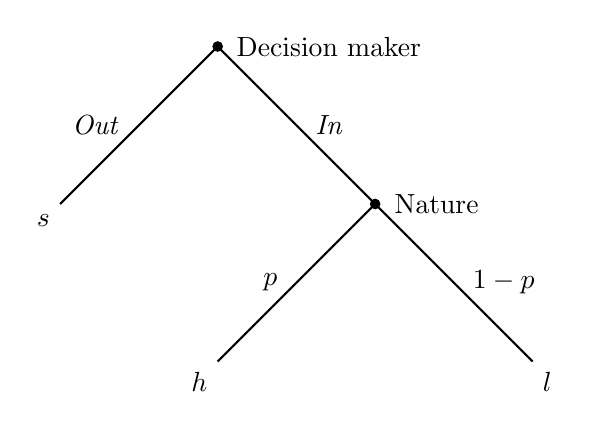
\begin{tikzpicture}[scale=2]
		\node[right] at (0,2) {~Decision maker};
		\draw[-, thick] (0,2) -- (-1,1) node[below left] {$s$};
		\node[left] at (-0.5,1.5) {\emph{Out}~~};
		\draw [fill] (0,2) circle [radius=0.03];
		\draw[-, thick] (0,2) -- (1,1) node[right] {~Nature};
		\node[right] at (0.5,1.5) {~\emph{In}};
		\draw [fill] (1,1) circle [radius=0.03];
		\draw[-, thick] (1,1) -- (0,0) node[below left] {$h$};
		\node[left] at (0.5,0.5) {$p$~~};
		\draw[-, thick] (1,1) -- (2,0) node[below right] {$l$};
		\node[right] at (1.5,0.5) {~$1-p$};		
	\end{tikzpicture}
\end{center}

In the following we look at different benchmarks.
In particular, we are interested in whether and how the optimal minimum acceptable probability MAP$^*$ depends on the distribution of $p$.


\subsection{Expected utility theory}
\label{subsec:EUT}

Assume the DM to have a utility function $U(\cdot)$. 
In an expected utility framework, utility is strictly increasing with outcome.
Hence, we have 
\begin{align}
	U(l) < U(s) < U(h)
\end{align}

In this appendix, we consider the MAP as a probability i.e. MAP $\in [0,1]$. The DM wants to choose his MAP such that he maximizes his expected utility $U($\textit{MAP}$)$ which is
\begin{align}
	U(\textit{MAP}) &= \int_{p=0}^{\textit{MAP}} f(p) \cdot U(s) \, dp %%%
	+ \int_{p=\textit{MAP}}^1 f(p) \cdot \left[p \cdot U(h) + (1-p) \cdot U(l) \right] dp \\
	     &= \int_{p=0}^{\textit{MAP}} f(p) \cdot U(s) \, dp %%%
	     - \int_{p=1}^{\textit{MAP}} f(p) \cdot \left[p \cdot U(h) + (1-p) \cdot U(l) \right] dp 
\end{align}

We use the Fundamental Theorem of Calculus to derive the first order condition:\footnote{
From the differentiability of $U(.)$ and $\frac{\partial U(\textit{MAP})}{\partial \textit{MAP}} (0) > 0 $ and $\frac{\partial U(\textit{MAP})}{\partial \textit{MAP}} (1) < 0$, we can conclude that at least one local maximum exists.
If the solution of the FOC is unique, then it must be this maximum.
}
\begin{align}
	\frac{\partial U(\textit{MAP})}{\partial\textit{MAP}} %%%
	= f(\textit{MAP}) \cdot U(s) - f(\textit{MAP}) \cdot \left[\textit{MAP} \cdot U(h) + (1-\textit{MAP}) \cdot U(l) \right] \stackrel{!}{=} 0
\end{align}

The density function $f(p)$ has full support.
Therefore, $f(\textit{MAP})$ is positive and we can simplify the expression to 
\begin{align}
	\textit{MAP}^* = \frac{U(s)-U(l)}{U(h)-U(l)}
\end{align}

The optimal MAP$^*$ is independent of the distribution of $p$.
Thus, an expected utility maximizer should not be influenced by it. 


\subsection{Outcome-based add-ons}

The result of Section \ref{subsec:EUT} holds if the utility function of the DM is extended by other elements that are based on outcomes.
For example, the DM might receive extra \mbox{(dis-)} utility from playing the lottery.
Or he might feel additional happiness or regret in case the outcome of the lottery is high or low, respectively.
Such add-ons to the utility function lead to a different MAP$^*$, but $f(p)$ would still cancel out of the first order condition.
Hence, MAP$^*$ should still be independent of the distribution of $p$.  


\subsection{Probability weighting}

Experimental evidence shows that humans have difficulties in handling probablities.
In particular, they seem to overestimate small probabilities and underestimate large ones.\footnote{
Back in 2000, \citet[p.~348--349]{Starmer2000} mentioned research spanning 50 years which supports this.
This still holds true today, e.g. see \citet[Figure 4 on p.~276]{Li2020a}.  
} 
In the following we assume the DM to have a continuous probability weighting function $w: [0,1] \rightarrow [0,1]$ with $w(0) = 0$ and $w(1) = 1$.
This gives the DM the following utility function:\footnote{
Probability weighting is not compatible with the axiomatic framework of expected utility theory.
We use the notion of utility in a broad sense covering also non-expected utility theories.
}
\begin{align}
	U(\textit{MAP}) &= \int_{p=0}^{\textit{MAP}} f(p) \cdot U(s) \, dp %%%
	+ \int_{p=\textit{MAP}}^1 f(p) \cdot \left[w(p) \cdot U(h) + w(1-p) \cdot U(l) \right] dp
\end{align}

This leaves us with the FOC:
\begin{align}
	\label{eq:FOCsimplified}
	U(s) - \left[w(\textit{MAP}) \cdot U(h) + w(1-\textit{MAP}) \cdot U(l) \right] = 0 
\end{align}

From the assumptions about the weighting function and $U(l)<U(s)<U(h)$, it follows that this equation has at least one solution (Bolzano's Theorem).
As in Section \ref{subsec:EUT}, all solutions are independent of the distribution of $p$.\footnote{
We may get to a unique solution of equation (\ref{eq:FOCsimplified}) if we place additional requirements on the outcomes $U(\cdot)$ and/or on $w(p)$.
Two possibilities are:
1.) A unique solution is guaranteed if $w(p)$ is strictly increasing and symmetric, i.e. $w(1-p) = 1-w(p)$ or
2.) A unique solution is guaranteed if $w(p)$ is strictly increasing and the utility of the low outcome including all possible add-ons is set to zero, i.e. $U(l) = 0$.
}\textsuperscript{,} 
\footnote{
In case of multiple solutions, we assume the distribution of $p$ does not offer cues which lead to selecting a different optimum MAP in each treatment.
}
	

\subsection{Rank-dependent utility}
\label{subsec:RDU}
%Let $p^*$ be the frequency of the high payoff, whose distribution varies between treatments.
%Since we expect that attitudes towards complex risk might make participants state different MAPs in the three treatments, we adapt the toy example in \cite{Li2020a} and make the following assumptions:
In this section, we present the assumptions we made in order to derive the hypothesis.
Unlike in the previous appendices, we focus on a numerical calculation.

We adapt the toy example in \cite{Li2020a} and make the following assumptions:
\begin{itemize}
\item The utility of outcomes is fixed. We consider $U(high) = U(\pounds4) = 1$, $U(low) = U(\pounds1) = 0$, and $U(safe) = U(\pounds2) = 1/3$.\footnote{
%We set the utility of the safe payoff such that $U(high) > U(safe) > U(low)$.
%$U(safe) = 1/3$ is the value of the safe payoff for which a risk neutral first mover is indifferent between the lottery with these high and low payoffs, and the safe payoff.
%
%Given our parameters (further in this section), a necessary condition for the optimal MAPs to differ in the three treatments is that $U(safe) \in [0.296, 0.516]$.
%If $U(safe) \in [0.146, 0.296) \cup (0.516, 0.641]$, two of the three optimal MAPs are equal and the third one is different.
%If $U(safe) \in [0, 0.146) \cup (0.641, 1]$, all three optimal MAPs are equal.
%%We set the utility of the safe payoff such that $U(\pounds2) = x \times U(\pounds4) + (1-x) \times U(\pounds1)$, where $x \in [0,1]$.
%%This leads to $x^* = 1/3$.
$U(safe)=1/3$ was chosen because, given the data on betrayal aversion, it makes a mildly risk-averse player indifferent between accepting any lottery and the safe payoff.
}
\item Participants use a probability weighting function because they perceive the tasks to involve complex risks. Similar to \cite{Li2020a}, we use \citeauthor{Prelec1998}'s (\citeyear{Prelec1998}) \textit{compound invariance} function:
$$w(p) = (exp(-(-ln(p))^\alpha))^\beta$$ 
\item We use $\alpha = 0.65$ and $\beta = 1.0467$, which according to \cite{Li2020a} are the most common values for risky probability weighting.
\item Participants use ``forward'' evaluation: they consider the three possible outcomes and take into account their probabilities, as resulting from the probability weighting function above.
\item Participants have the following rank-dependent utility function \citep{Schmeidler1989}, in which an act generated by a choice of MAP leads to:
$$RDU = w(P(\pounds4)) \cdot 1 + (w(P(\pounds4) + P(\pounds2)) - w(P(\pounds4))) \cdot (1/3)$$
where $P(\pounds4)$ is the probability of receiving the high payoff for a certain MAP in the respective treatment, $P(\pounds2)$ the probability of receiving the safe payoff, and $P(\pounds1)$ the probability of receiving the low payoff (which does not appear in the utility function, as the utility of the low payoff is considered to be 0).
\end{itemize}

In this case, the MAPs which maximize participants' utility in the three treatments are: $MAP^{*}_G = 7 (RDU = 0.628)$, $MAP^{*}_U = 8 (RDU = 0.495)$, and $MAP^{*}_B = 9 (RDU = 0.439)$.

\newpage
\section{Range-frequency model: a numerical example}
\label{section:appendixb}
\setcounter{figure}{0}
\setcounter{table}{0}
\renewcommand{\thefigure}{B.\arabic{figure}}
\renewcommand{\thetable}{B.\arabic{table}}
According to the range-frequency model, participants categorize stimuli according to range and frequency, and then evaluate them based on a compromise between the two ways of classification.

Let us assume that a participant uses four bins to categorize stimuli: bad lotteries, not OK lotteries, OK lotteries, and good lotteries.
When using the range criterion, this participant bins existing lotteries in all treatments in the following way:
\begin{center}
\begin{tabular}{p{3cm} c}
Category & Dark blue sectors \\
\hline
Bad & 0, 1, 2, 3\\
Not OK & 4, 5, 6, 7\\
OK & 8, 9, 10, 11\\
Good & 12, 13, 14, 15\\
\hline
\end{tabular}
\end{center}

If she bins lotteries according to frequency, she arrives at the following division in each treatment:
\begin{center}
\begin{tabular}{p{3cm} c}
Category & Dark blue sectors \\
\hline
& The Good \\
\cmidrule{2-2}
Bad & 0, 1, 2, 3, 4, 5, 6, 7\\
Not OK & 8, 9, 10, 11, 12\\
OK & 13, 14\\
Good & 15\\
\cmidrule{2-2}
& The Uniform \\
\cmidrule{2-2}
Bad & 0, 1, 2, 3\\
Not OK & 4, 5, 6, 7\\
OK & 8, 9, 10, 11\\
Good & 12, 13, 14, 15\\
\cmidrule{2-2}
& The bad \\
\cmidrule{2-2}
Bad & 0\\
Not OK & 1, 2\\
OK & 3, 4, 5, 6, 7\\
Good & 8, 9, 10, 11, 12, 13, 14, 15\\
\hline
\end{tabular}
\end{center}

If she thinks only categories OK and Good are acceptable and compromises between the two divisions of stimuli, she could report the following MAPs: MAP\textsubscript{G} = 10.5, MAP\textsubscript{U} = 8, MAP\textsubscript{B} = 5.5.
As she gives more weight to the frequency criterion, choices get closer to one another.

\newpage
\section[Instructions]{Instructions\footnote{
While the instructions look slightly differently in Qualtrics, we strove to depict the visual elements (the wheels, the distributions) as accurately as possible in this section.
The horizontal lines mark the separation between pages.
}}
\label{section:appendixc}
\setcounter{figure}{0}
\setcounter{table}{0}
\renewcommand{\thefigure}{C.\arabic{figure}}
\renewcommand{\thetable}{C.\arabic{table}}

\textbf{Statement of consent}\\
\\
\noindent In this study, you will be asked to make decisions.
You will also be asked to answer comprehension questions, reasoning questions, and questions about yourself.
Your data will remain anonymous in accordance with GDPR (the European Union's personal data protection law).\\
\\
\noindent This study follows the guidelines of the BEELab at Maastricht University.
This means that all information you receive during the study is truthful.\\
\\
\noindent To continue, please select ``I agree to participate".
\begin{itemize}
\item I agree to participate
\item I don't agree to participate
\end{itemize}

\bigskip
\noindent \rule{\linewidth}{0.4pt}

\noindent Before you start, please switch off your phone/e-mail/music so you can focus on this study.
Thank you!

\noindent Please enter your Prolific ID: \rule{1cm}{0.15mm}

\bigskip
\noindent \rule{\linewidth}{0.4pt}

\noindent \textbf{Part 1}

\noindent This part explains what the study is about and presents examples.
We will test your understanding of the situation with some questions.

\noindent To continue to Part 2, you have to answer these questions correctly.

\bigskip
\noindent \rule{\linewidth}{0.4pt}

\noindent Consider a wheel of fortune like the one below.\phantomsection\label{explanation}
The wheel is equally likely to land on each sector.
The pointer indicates the result: it's the sector which ends up at 12 o'clock when the wheel stops spinning.
Give it a try!

\begin{figure}[h!]
	\centering
	{\includegraphics[width=0.4\linewidth]{SpinMe.pdf}}
\end{figure}

\bigskip
\noindent \rule{\linewidth}{0.4pt}

\noindent In Part 2, you will see more such wheels. All wheels have \textbf{15 sectors} in total, which are either light blue or dark blue.
The number in the middle is the \textbf{number of dark blue sectors} in a wheel.
 
\noindent Below is an example with five wheels.

\begin{figure}[h!]
	\centering
	{\includegraphics[width=\linewidth]{Explaining_MAP.pdf}}
\end{figure}

\noindent \textbf{One} of the wheels will be randomly selected. Each wheel is \textbf{equally likely} to be selected. If the selected wheel is spun, it is {equally likely to land on each sector}.

\noindent You will have the following options for your bonus:

\begin{figure}[h!]
	\centering
	{\includegraphics[width=\linewidth]{Options.pdf}}
\end{figure}

\noindent Let us consider some examples. If the selected wheel has
\begin{itemize}
\item 15 dark blue sectors, if you \textbf{SPIN} it your bonus is £4.00 for sure.
If you \textbf{DON'T SPIN} it, you are guaranteed to receive £2.00.
\item 0 dark blue sectors, if you \textbf{DON'T SPIN} it you are guaranteed £2.00.
If you \textbf{SPIN} it, your bonus is £1.00 for sure.
\end{itemize}

\noindent \textbf{Without knowing} which wheel has been selected, you will be asked which wheels you want to \textbf{SPIN} for your bonus, and which ones you \textbf{DON'T} want to \textbf{SPIN}.

\bigskip
\noindent \rule{\linewidth}{0.4pt}

\noindent You will be asked the following question:

\begin{mdframed}[backgroundcolor=LightBlue, linecolor=white]
\noindent \textit{Which wheels do you prefer to SPIN for your bonus?} \\
\\
\noindent \textit{I prefer to SPIN wheels which have at least \framebox[0.1\textwidth]{\rule{0pt}{15pt}} dark blue sectors.} \\
\\
\noindent \textit{If the randomly selected wheel has \textbf{fewer than … dark blue sectors}, I \textbf{DON’T SPIN} it.
I receive £2.00.} \\
\textit{If the randomly selected wheel has \textbf{… or more dark blue sectors}, I \textbf{SPIN} it.
I receive £4.00 if the wheel lands on dark blue, and £1.00 if it lands on light blue.}
\end{mdframed}

\noindent You can practice by introducing integers between 0 and 15 in the box above.
When you introduce a number, all wheels with fewer dark blue sectors than your answer will be grayed out, indicating that you prefer DON'T SPIN for those wheels.
The wheels with the same number or more dark blue sectors than your answer will not be affected, indicating that you prefer SPIN if one of those wheels is selected.

\noindent At the end of the study you will be told which wheel has been selected.
Its number of dark blue sectors will be compared to your answer, and your bonus will be determined by the relevant option (SPIN or DON'T SPIN).\phantomsection\label{end}

\noindent Your \textbf{input on this screen} is simply for you to practice and it \textbf{doesn't affect your bonus}.
You \textbf{don't have to memorize} this explanation: a non-interactive version like the one linked below under ``View explanation" will be available whenever relevant.

\noindent \textcolor{blue}{\underline{View explanation}}

\bigskip
\noindent \rule{\linewidth}{0.4pt}

\noindent The comprehension questions will start on the next screen.

\bigskip
\noindent \rule{\linewidth}{0.4pt}

\noindent \underline{Comprehension Question 1}

\begin{figure}[h!]
	\centering
	{\includegraphics[width=\linewidth]{five_wheelsS1_15.pdf}}
\end{figure}
 
\noindent Consider the wheels above.
Let's assume you stated that you want to SPIN wheels with at least 3 sectors for your bonus.
For this reason, wheels with fewer than 3 sectors are grayed out.
The wheel with 7 sectors has been randomly selected (the wheel with a black border).\\
\\
\noindent Please select \textbf{all that apply}.\\
 \\
\noindent \textcolor{blue}{\underline{View explanation}}\footnote{
Upon clicking, a pdf document opened in a separate window.
The document contained the text on page \pageref{explanation} (``Consider a wheel...'') up to page \pageref{end} (``... determined by the relevant option (SPIN or DON'T SPIN).'').
}\\
\begin{itemize}
\item[$\square$] I DON'T SPIN the selected wheel.
\item[$\square$] I SPIN the selected wheel.
\item[$\square$] My bonus is £1.00.
\item[$\square$] My bonus is £2.00.
\item[$\square$] My bonus is £4.00 if the selected wheel lands on dark blue, £1.00 if it lands on light blue.
\item[$\square$] My bonus is £1.00 if the selected wheel lands on dark blue, £2.00 if it lands on light blue.
\end{itemize}

\noindent \rule{\linewidth}{0.4pt}
\newpage
\noindent \underline{Comprehension Question 2}

\begin{figure}[h!]
	\centering
	{\includegraphics[width=\linewidth]{five_wheelsS2_15.pdf}}
\end{figure}
 
\noindent Consider the wheels above.
Let's assume you stated that you want to SPIN wheels with at least 8 sectors for your bonus.
For this reason, wheels with fewer than 8 sectors are grayed out.
The wheel with 7 sectors has been randomly selected (the wheel with a black border).\\
\\
\noindent Please select \textbf{all that apply}.\\
 \\
\noindent \textcolor{blue}{\underline{View explanation}}\footnote{
Upon clicking, a pdf document opened in a separate window.
The document contained the text on page \pageref{explanation} (``Consider a wheel...'') up to page \pageref{end} (``... determined by the relevant option (SPIN or DON'T SPIN).'').
}\\
\begin{itemize}
\item[$\square$] I DON'T SPIN the selected wheel.
\item[$\square$] I SPIN the selected wheel.
\item[$\square$] My bonus is £1.00.
\item[$\square$] My bonus is £2.00.
\item[$\square$] My bonus is £4.00 if the selected wheel lands on dark blue, £1.00 if it lands on light blue.
\item[$\square$] My bonus is £1.00 if the selected wheel lands on dark blue, £2.00 if it lands on light blue.
\end{itemize}

\noindent \rule{\linewidth}{0.4pt}
\newpage
\noindent \underline{Comprehension Question 3}\footnote{
If participants answered all comprehension questions correctly, they would go to the next part.
If not, they were given the chance to review their answers.
Those who revised correctly would also go to the next part.
The experiment ended for those who did not revise correctly.
}
 
\noindent Please select the correct statement from each of the following pairs.

\begin{tasks}[style=itemize](2)
\task Each wheel is \textbf{equally likely} to be selected.
\task Some wheels are \textbf{more likely} to be selected than others.
\task I \textbf{can} influence the chance that a particular wheel is selected.
\task I \textbf{can't} influence the chance that a particular wheel is selected. 
\task I get to spin the selected wheel \textbf{regardless of} whether it is in the grayed out area or not.
\task I get to spin the selected wheel \textbf{only if} it's not in the grayed out area.
\task If I get to spin the selected wheel, it is \textbf{equally likely} to land on each sector.
\task If I get to spin the selected wheel, it is \textbf{more likely} to land on sectors which are initially around 12 o'clock. 
\task My bonus is £4.00 if the selected wheel is in the \textbf{grayed out} area and the selected wheel lands on \textbf{light blue}.
\task My bonus is £4.00 if the selected wheel is in the \textbf{non-grayed out} area and the selected wheel lands on \textbf{dark blue}.
\end{tasks}

\bigskip
\noindent \rule{\linewidth}{0.4pt}

\noindent You have answered all questions in Part 1 correctly. \\
You will now be directed to Part 2.

\bigskip
\noindent \rule{\linewidth}{0.4pt}

\noindent \textbf{Part 2}\footnote{
The decisions on the next three screens were shown in randomized order.
}

\noindent In this part, you will be asked 
\begin{itemize}
\item How you want your bonus to be determined \textbf{in three different situations}.
Choose your most preferred option from those available.
There are no right or wrong answers to these questions.
\item Reasoning questions and questions about yourself.
\end{itemize}

\noindent At the end of Part 2, \textbf{one of the three situations will be randomly selected}, and your bonus will be determined according to your answer in that situation.
Each of the three situations is equally likely to be selected.

\noindent \rule{\linewidth}{0.4pt}

\newpage
\begin{figure}[h!]
	\centering
	{\includegraphics[width=\linewidth]{Left_15.pdf}}
\end{figure}

\noindent Consider the wheels above.
Which wheels do you prefer to SPIN for your bonus?\\
{\small Please enter an integer between 0 and 15.} \\
\\
\noindent I prefer to SPIN wheels which have at least \framebox[0.1\textwidth]{\rule{0pt}{15pt}}\footnote{
The box was dynamic: as participants typed a number, the wheels which were ineligible for being selected in case that number was the participant's decision were grayed out and the ellipses below were replaced with that number.
This way, participants were informed about the implications of potential decisions.
}
dark blue sectors.\\
\\
\noindent If the randomly selected wheel has fewer than ... dark blue sectors, I DON'T SPIN it.
My bonus is £2.00.

\noindent If the randomly selected wheel has ... or more dark blue sectors, I SPIN it.
My bonus is
\begin{itemize}
\item £1.00 if the selected wheel lands on light blue, and
\item £4.00 if it lands on dark blue.
\end{itemize}

\noindent \rule{\linewidth}{0.4pt}

\newpage
\begin{figure}[h!]
	\centering
	{\includegraphics[width=\linewidth]{Uniform_15.pdf}}
\end{figure}

\noindent Consider the wheels above.
Which wheels do you prefer to SPIN for your bonus?\\
{\small Please enter an integer between 0 and 15.} \\
\\
\noindent I prefer to SPIN wheels which have at least \framebox[0.1\textwidth]{\rule{0pt}{15pt}} dark blue sectors.\\
\\
\noindent If the randomly selected wheel has fewer than ... dark blue sectors, I DON'T SPIN it.
My bonus is £2.00.

\noindent If the randomly selected wheel has ... or more dark blue sectors, I SPIN it.
My bonus is
\begin{itemize}
\item £1.00 if the selected wheel lands on light blue, and
\item £4.00 if it lands on dark blue.
\end{itemize}

\noindent \rule{\linewidth}{0.4pt}

\newpage
\begin{figure}[h!]
	\centering
	{\includegraphics[width=\linewidth]{Right_15.pdf}}
\end{figure}

\noindent Consider the wheels above.
Which wheels do you prefer to SPIN for your bonus?\\
{\small Please enter an integer between 0 and 15.} \\
\\
\noindent I prefer to SPIN wheels which have at least \framebox[0.1\textwidth]{\rule{0pt}{15pt}} dark blue sectors.\\
\\
\noindent If the randomly selected wheel has fewer than ... dark blue sectors, I DON'T SPIN it.
My bonus is £2.00.

\noindent If the randomly selected wheel has ... or more dark blue sectors, I SPIN it.
My bonus is
\begin{itemize}
\item £1.00 if the selected wheel lands on light blue, and
\item £4.00 if it lands on dark blue.
\end{itemize}

\noindent \rule{\linewidth}{0.4pt}

\newpage
The reasoning questions and the questions about yourself will start on the next screen.

\smallskip
\noindent \rule{\linewidth}{0.4pt}

\begin{figure}[h!]
	\centering
	{\includegraphics[width=\linewidth]{Ambiguous_15.pdf}}
\end{figure}

\noindent The scenario described below is \textbf{hypothetical}: your answer \textbf{doesn't influence your bonus}.
\smallskip
\noindent Imagine 32 wheels of fortune with 15 sectors each.
Like before, their sectors are either light blue (worth £1.00) or dark blue (worth £4.00).
However, the sectors' color is hidden, so you \textbf{don't know how many dark blue} or \textbf{light blue sectors} each wheel has.
One of the 32 wheels will be selected at random: depending on your answer to the question below, you SPIN the wheel or you DON'T SPIN it.
 
\noindent In this case, which wheels would you prefer to SPIN for your bonus?

\noindent {\small Please enter an integer between 0 and 15.}

\smallskip
\noindent I prefer to SPIN wheels which have at least \framebox[0.1\textwidth]{\rule{0pt}{15pt}} dark blue sectors.

\smallskip
\noindent If the randomly selected wheel has fewer than ... dark blue sectors, I DON'T SPIN it.
My bonus is £2.00.

\noindent If the randomly selected wheel has ... or more dark blue sectors, I SPIN it.
My bonus is
\begin{itemize}
\item £1.00 if the selected wheel lands on light blue, and
\item £4.00 if it lands on dark blue.
\end{itemize}

\noindent \rule{\linewidth}{0.4pt}

\newpage
\noindent Please answer the following questions.\\
\\
\noindent Simon had 17 plants at home and all but 8 died.
How many are left?\\
\framebox[0.1\textwidth]{\rule{0pt}{15pt}}

\noindent Claire's grandmother has three granddaughters.
The first two are named April and May.
What is the third granddaughter's name?\\
\framebox[0.1\textwidth]{\rule{0pt}{15pt}}

\noindent If you're running a race and you pass the person in second place, what place are you in? (type in the number of the place)\\
\framebox[0.1\textwidth]{\rule{0pt}{15pt}}

\noindent A scientist grows bacteria on a Petri dish.
Every day, the area covered by bacteria doubles in size.
If it takes 6 days for the entire dish to be covered, how long would it take for half of the dish to be covered?\\
\framebox[0.1\textwidth]{\rule{0pt}{15pt}}

\bigskip
\noindent \rule{\linewidth}{0.4pt}

\noindent What subject did you study for your most recent degree? \textit{[drop-down menu]}\\
\\
\noindent How do you see yourself: are you generally a person who is fully prepared to take risks or do you try to avoid taking risks?
\begin{figure}[h!]
	\centering
	{\includegraphics[width=\linewidth]{RiskAversion.pdf}}
\end{figure}

\bigskip
\noindent \rule{\linewidth}{0.4pt}

\noindent Which of the following do you take into consideration when deciding whether to take part in a study?
Please select all that apply.\footnote{
One of the next two screens was shown at random to participants.
}
\begin{itemize}
\item Total pay
\item Pay per hour
\item Other things, such as \\
\framebox[\textwidth]{\rule{0pt}{15pt}}
\end{itemize}

\bigskip
\noindent \rule{\linewidth}{0.4pt}

\noindent The next questions are about general facts that you may or may not know.
Please give your best estimates.
We also ask that you please not look up the answers; we are interested in people's estimates, whether or not they are accurate.\\
\\
Do you think that the \textbf{average daily temperature in June} in Amsterdam, the Netherlands, between 1971 and 2020 was higher or lower than 14°C?
\begin{itemize}
\item Higher
\item Lower
\end{itemize}
\leavevmode \\
\noindent What do you think was the \textbf{average daily temperature in June} in Amsterdam in this period?\\
\framebox[0.1\textwidth]{\rule{0pt}{15pt}}°C\\
\\
\noindent Do you think that the number of \textbf{average daily hours of sunshine in June} in Amsterdam, the Netherlands, between 1971 and 2020 was higher or lower than 10?
\begin{itemize}
\item Higher
\item Lower
\end{itemize}
\leavevmode \\
\noindent What do you think was the number of \textbf{average daily hours of sunshine in June} in Amsterdam in this period?\\
\framebox[0.1\textwidth]{\rule{0pt}{15pt}} hour(s) and \framebox[0.1\textwidth]{\rule{0pt}{15pt}} minute(s)

\bigskip
\noindent \rule{\linewidth}{0.4pt}

\noindent The next questions are about general facts that you may or may not know.
Please give your best estimates.
We also ask that you please not look up the answers; we are interested in people's estimates, whether or not they are accurate.\\
\\
Do you think that the \textbf{average daily temperature in June} in Amsterdam, the Netherlands, between 1971 and 2020 was higher or lower than 17°C?
\begin{itemize}
\item Higher
\item Lower
\end{itemize}
\leavevmode \\
\noindent What do you think was the \textbf{average daily temperature in June} in Amsterdam in this period?\\
\framebox[0.1\textwidth]{\rule{0pt}{15pt}}°C\\
\\
\noindent Do you think that the number of \textbf{average daily hours of sunshine in June} in Amsterdam, the Netherlands, between 1971 and 2020 was higher or lower than 4?
\begin{itemize}
\item Higher
\item Lower
\end{itemize}
\leavevmode \\
\noindent What do you think was the number of \textbf{average daily hours of sunshine in June} in Amsterdam in this period?\\
\framebox[0.1\textwidth]{\rule{0pt}{15pt}} hour(s) and \framebox[0.1\textwidth]{\rule{0pt}{15pt}} minute(s)

\bigskip
\noindent \rule{\linewidth}{0.4pt}

\noindent For the questions below, please be as honest and accurate as you can throughout.
Try not to let your response to one statement influence your responses to other statements.
There are no ``correct" or ``incorrect" answers.
Answer according to your own feelings, rather than how you think ``most people" would answer.

\begin{table}[htbp]
\begin{tabular}
   {@{}
	l
	*5c
	@{}
	}
&\thead{I disagree\\a lot}&\thead{I disagree\\a little}&\thead{I neither\\agree nor\\disagree}&\thead{I agree a\\little}&\thead{I agree a\\lot}\\
\thead[vl]{In uncertain times, I\\usually expect the best.}	& $\ocircle$ & $\ocircle$ & $\ocircle$ & $\ocircle$ & $\ocircle$ \\
\thead[vl]{It's easy for me to relax.}	& $\ocircle$ & $\ocircle$ & $\ocircle$ & $\ocircle$ & $\ocircle$ \\
\thead[vl]{If something can go wrong for\\me, it will.}	& $\ocircle$ & $\ocircle$ & $\ocircle$ & $\ocircle$ & $\ocircle$ \\
\thead[vl]{I'm always optimistic about my\\future.}	& $\ocircle$ & $\ocircle$ & $\ocircle$ & $\ocircle$ & $\ocircle$ \\
\thead[vl]{I enjoy my friends a lot.}	& $\ocircle$ & $\ocircle$ & $\ocircle$ & $\ocircle$ & $\ocircle$ \\
\midrule
\addlinespace
&\thead{I disagree\\a lot}&\thead{I disagree\\a little}&\thead{I neither\\agree nor\\disagree}&\thead{I agree a\\little}&\thead{I agree a\\lot}\\
\thead[vl]{It's important for me to keep busy.}	& $\ocircle$ & $\ocircle$ & $\ocircle$ & $\ocircle$ & $\ocircle$ \\
\thead[vl]{I hardly ever expect things to go\\my way.}	& $\ocircle$ & $\ocircle$ & $\ocircle$ & $\ocircle$ & $\ocircle$ \\
\thead[vl]{I don't get upset too easily.}	& $\ocircle$ & $\ocircle$ & $\ocircle$ & $\ocircle$ & $\ocircle$ \\
\thead[vl]{I rarely count on good things\\happening to me.}	& $\ocircle$ & $\ocircle$ & $\ocircle$ & $\ocircle$ & $\ocircle$ \\
\thead[vl]{Overall, I expect more good\\things to happen to me than bad.}	& $\ocircle$ & $\ocircle$ & $\ocircle$ & $\ocircle$ & $\ocircle$ \\
\midrule
\addlinespace
&\thead{I disagree\\a lot}&\thead{I disagree\\a little}&\thead{I neither\\agree nor\\disagree}&\thead{I agree a\\little}&\thead{I agree a\\lot}\\
\thead[vl]{I would like to explore strange\\places.}	& $\ocircle$ & $\ocircle$ & $\ocircle$ & $\ocircle$ & $\ocircle$ \\
\thead[vl]{I like to do frightening things.}	& $\ocircle$ & $\ocircle$ & $\ocircle$ & $\ocircle$ & $\ocircle$ \\
\thead[vl]{I like new and exciting\\experiences, even if I have to\\break the rules.}	& $\ocircle$ & $\ocircle$ & $\ocircle$ & $\ocircle$ & $\ocircle$ \\
\thead[vl]{I prefer friends who are exciting\\and unpredictable.}	& $\ocircle$ & $\ocircle$ & $\ocircle$ & $\ocircle$ & $\ocircle$ \\
\bottomrule
\end{tabular}
\end{table}

\newpage
\noindent On the next screen, you will be informed\footnote{
Only one of the next two screens was shown to participants, depending on how their randomly chosen decision compared to the randomly selected wheel.
The examples illustrate the two possible scenarios.
}
\begin{itemize}
\item which of three situations has been selected, and
\item which wheel from that situation has been selected.
\end{itemize}
  
\bigskip  
\noindent \rule{\linewidth}{0.4pt}    

\noindent \textit{Situation 1: the selected wheel was eligible for spinning}\\
\\
\noindent The situation below has been randomly selected.
In this situation, you stated that you prefer to spin the wheel if it has \textbf{at least 6 dark blue sectors}.
The randomly selected wheel is the one surrounded by a black border.
Since this wheel is not grayed out (as it has 6 or more dark blue sectors), you will SPIN it for your bonus.
\begin{figure}[h!]
	\centering
	{\includegraphics[width=\linewidth]{Eligible.pdf}}
\end{figure}

\noindent \rule{\linewidth}{0.4pt}
\newpage
\noindent Spin the selected wheel to determine your bonus.
If you wish, you can try it out a couple of times before the final spin, which is the one that counts.
\begin{figure}[h!]
	\centering
	{\includegraphics[width=0.4\linewidth]{FinalSpin.pdf}}
\end{figure}

\noindent \rule{\linewidth}{0.4pt}
\newpage
\noindent \textit{Situation 2: the selected wheel was not eligible for spinning}\\
\\
\noindent The situation below has been randomly selected.
In this situation, you stated that you prefer to spin the wheel if it has \textbf{at least 6 dark blue sectors}.
The randomly selected wheel is the one surrounded by a black border.
Since this wheel is grayed out (as it has fewer than 6 dark blue sectors), you DON'T SPIN it.
Your bonus is £2.00.

\begin{figure}[h!]
	\centering
	{\includegraphics[width=\linewidth]{Ineligible.pdf}}
\end{figure}
		
\bigskip
\noindent \rule{\linewidth}{0.4pt}

\noindent We thank you for your time spent taking this survey.
Your response has been recorded.\\
\noindent If you have any comments, please write them in the box below. \\
\framebox[\textwidth]{\rule{0pt}{15pt}}\\
\\
If you would like to be informed about the earnings of all participants in this study, please select the option below.
We will send you the earnings distribution via Prolific no later than a week after the last submission.
\begin{itemize}
\item[$\square$] I would like to be informed about the earnings distribution in this study.
\end{itemize}

\end{document}